\chapter{Appendix A}\label{chap:appendixA}
\markboth{Appendix A}{}% To set left/right header

\begin{figure} [t]
    \centering
    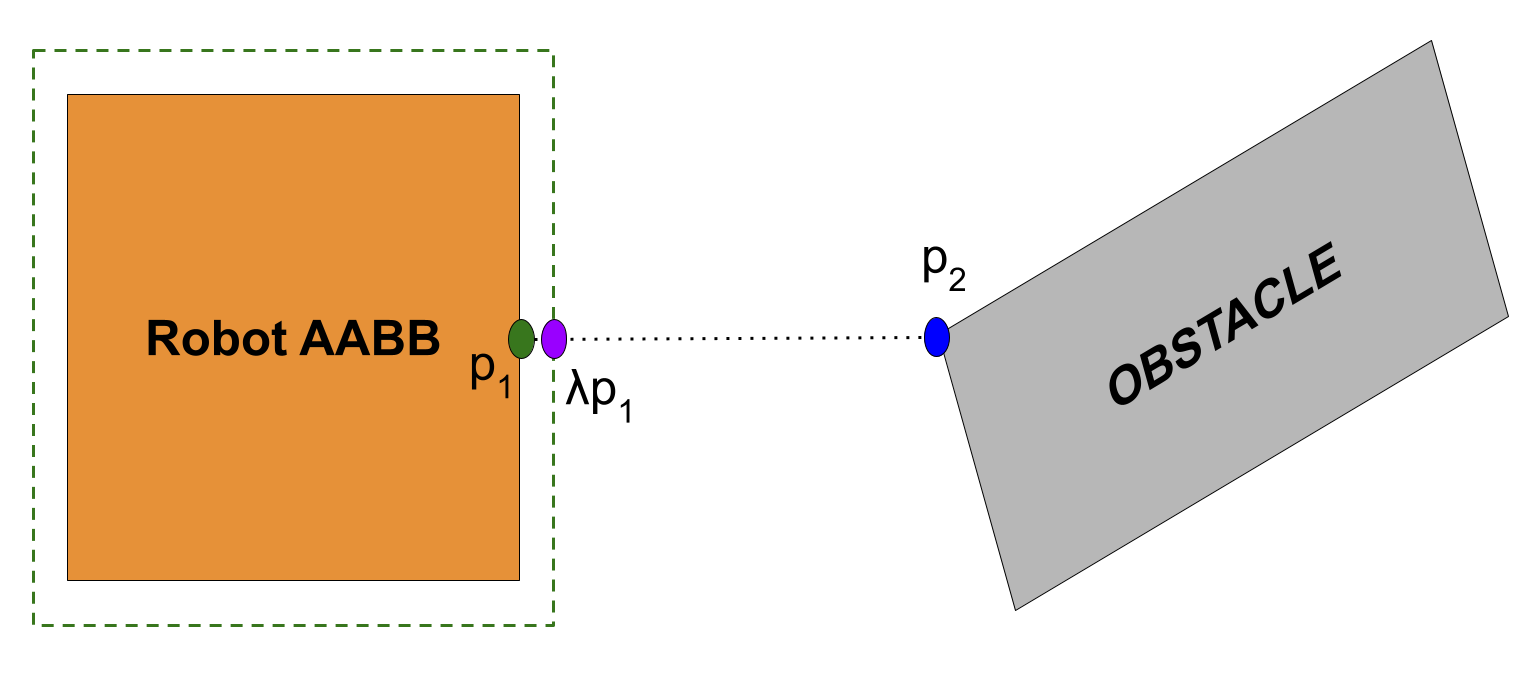
\includegraphics[width=0.8\linewidth]{figures/appendix/CCellipse.png}
    \caption{Collision checking given a uniform scaling of the robot AABB.}
    \label{fig:appendix_A}
\end{figure}

Given a current robot AABB, this proof aims to show that the closest point on the robot to an obstacle remains the closest point after uniform scaling, and that the closest point of the obstacle to the robot also remains unchanged (see Figure~\ref{fig:appendix_A}).

Let $A$ and $B$ be two convex sets. 
This assumption holds for the collision test presented in Section~\ref{sec:robust_CC} as the robot AABB is a convex shape, and the environment is decomposed into convex shapes.
Let \( p_1 \in A \) such that \( p_1 = \arg \min_{a \in A} \|a - b\| \, \forall b \in B \), and \( p_2 \in B \) such that \( p_2 = \arg \min_{b \in B} \|a - b\| \, \forall a \in A \).
Also let $\lambda A, \lambda \geq 1$ be a uniform scaling of $A$.

One want to show that:
\begin{enumerate}
    \item The projection of $p_1$ due to the scaling remains the closest point to the obstacle.
    \item $p_2$ remains the closest point to the projection of $p_1$. 
\end{enumerate}
\[
    \left\{
    \begin{aligned}
        \lambda p_1 &= \argmin_{a \in A} \|\lambda a - b\| \, \forall b \in B \\
        p_2 &= \argmin_{b \in B} \|\lambda p_1 - b\|
    \end{aligned}
    \right.
\]

\paragraph{1.}
Let \( a \in A \) and \( b \in B \).
One can express the following relationship:
\[
\|\lambda a - b\| = \lambda \left\|a - \frac{b}{\lambda}\right\|,
\]
where \(\frac{b}{\lambda} \in B\) because \(B\) is convex. 
Therefore, one gets:
\[
\arg \min_{a \in A} \left\|a - \frac{b}{\lambda}\right\| = \arg \min_{a \in A} \|a - b\| = p_1,
\]
which implies:
\[
\arg \min_{a \in A} \|\lambda a - b\| = \lambda p_1.
\]

\paragraph{2.}
Let \( b \in B \), \( b \neq p_2 \) such that:

\[
\|\lambda p_1 - b\|^2 = \|\lambda p_1 - p_2\|^2 + \|p_2 - b\|^2,
\]
and since \( p_2 \neq b \), one gets \( \|p_2 - b\|^2 > 0 \). 
Therefore, \( \|\lambda p_1 - b\| > \|\lambda p_1 - p_2\| \), which implies \( \arg \min_{b \in B} \|\lambda p_1 - b\| = p_2 \).

